\documentclass{article} 

\usepackage{graphicx}

\usepackage{mdframed}
\usepackage{listings,lstautogobble}
\usepackage{hyperref}
\usepackage{amsfonts}
\usepackage{amsmath}

\graphicspath{img}

\title{CSE160 Homework 4}
\author{Elijah Hantman}

%\renewcommand{\spn}[1]{\langle #1 \rangle}

\setlength{\emergencystretch}{10pt}

\begin{document}
    \maketitle

    {\large View and Projection}
    \begin{enumerate}
        \item What matrix is created by LookAt(eye=[0,0,2], at=[0,0,0], up=[0,1,0])? Is there a
            way to get this matrix using translate and/or rotate and/or scale? Explain

            \begin{mdframed}
               The matrix places the point $0,0,2$ at the origin,
               and orients the transformed origin point $0,0,0$ to
               sit at $0,0,1$. Finally the up vector ensures
               that the point $0,1,2$ ends up at $0,1,0$.


               To replicate this matrix first you translate $0,0,2$
               to the origin. Then you rotate so that $0,1,0$ lands
               on $0,1,0$ and $0,0,-2$ ends up at $0,0,2$.
            \end{mdframed}

        \item Illustrate the difference between orthographic (parallel) and perspective projection.
            \begin{mdframed}
                The main difference between perspective projection
                and orthographic projection is that orthographic projection
                places a constant in the w component while the perspective
                projection puts the depth in the w component. This means
                that when the hardware does a perspective divide the orthographic
                projection does not have perspective while the perspective projection
                makes objects further ways smaller.

                Conceptually we can imagine the region each projection will
                put into the unit cube to be rendered. For orthographic projections
                this region is a rectangular prism meaning things further away
                from the origin are projected to the same size as things close by.

                On the other hand, perspective projections have whats called
                a frustum which is a cut off rectangular pyramid. When the shape
                is transformed into a unit cube the things further away are shrunk
                down compared to things near by.
            \end{mdframed}

            \break
        \item Consider the 3D solid cube, with a cube-shaped notch removed from one corner.
            \begin{figure}[ht]
                \begin{center}
                    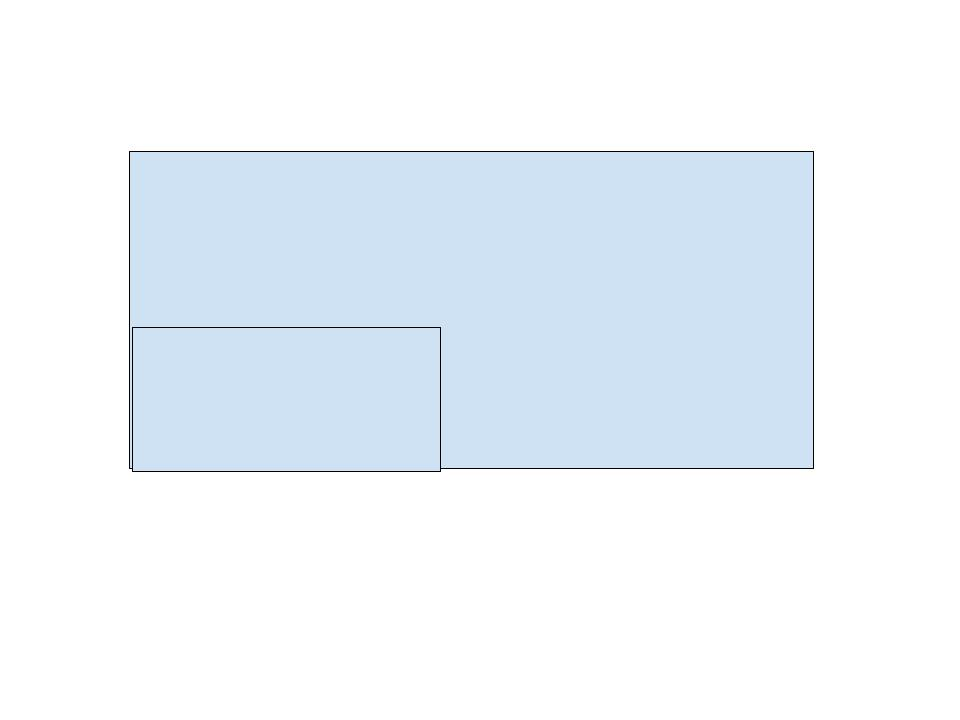
\includegraphics[scale=0.20, angle = 0]{img/ortho.jpg}
                    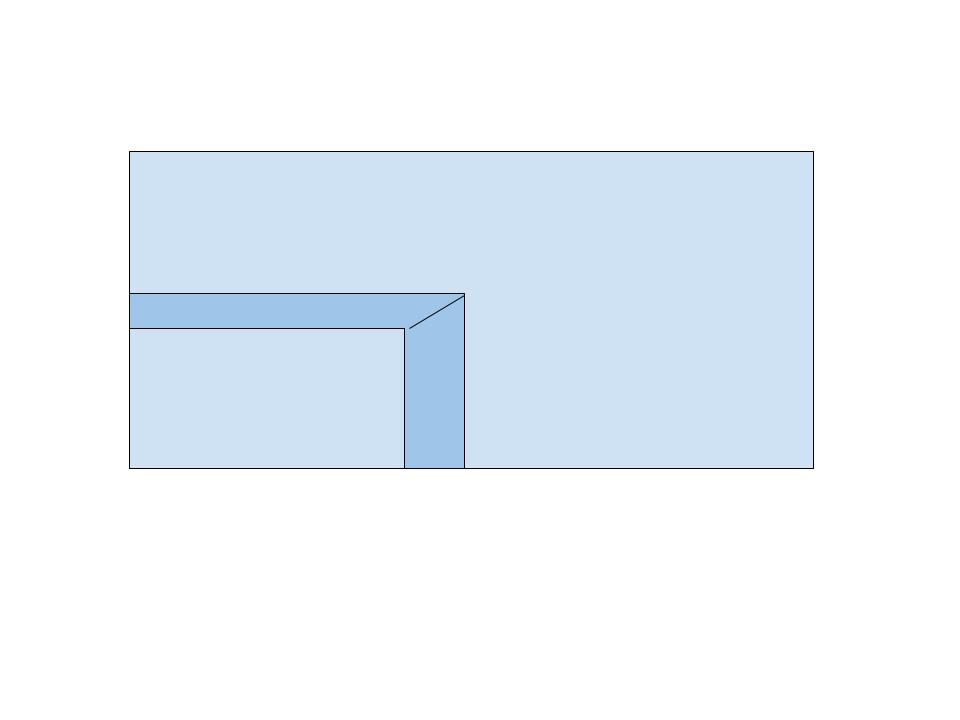
\includegraphics[scale=0.20, angle = 0]{img/perspective.jpg}
                \end{center}
            \end{figure}
            \begin{mdframed}
                The top is orthographic, as can be seen by the walls
                being parallel to the camera view.

                The second is perspective and that can be seen by the walls
                not being parallel due to perspective distortion.
            \end{mdframed}

        \item Suppose we set up a camera using LookAt eye=[2,4,3], at=[2,4,4], up=[0,1,0] and
            render a scene with two spheres of radius 1, centered at [2,4,5] and [2,10,8].

            \begin{enumerate}
                \break
                \item Draw this scene in 2D both on the x-z plane (left) and on the y-z plane (right).
                    Label the eye and the at points as well as the two spheres.
                    \begin{figure}[ht]
                        \begin{center}
                            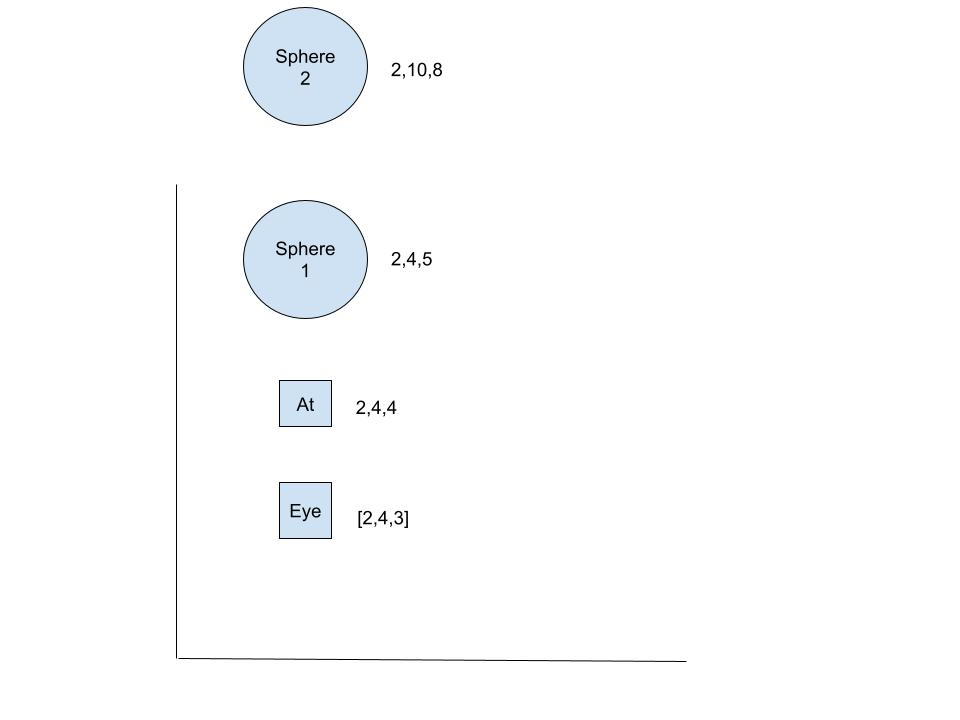
\includegraphics[scale=0.20, angle = 0]{img/xz_diag.jpg}
                            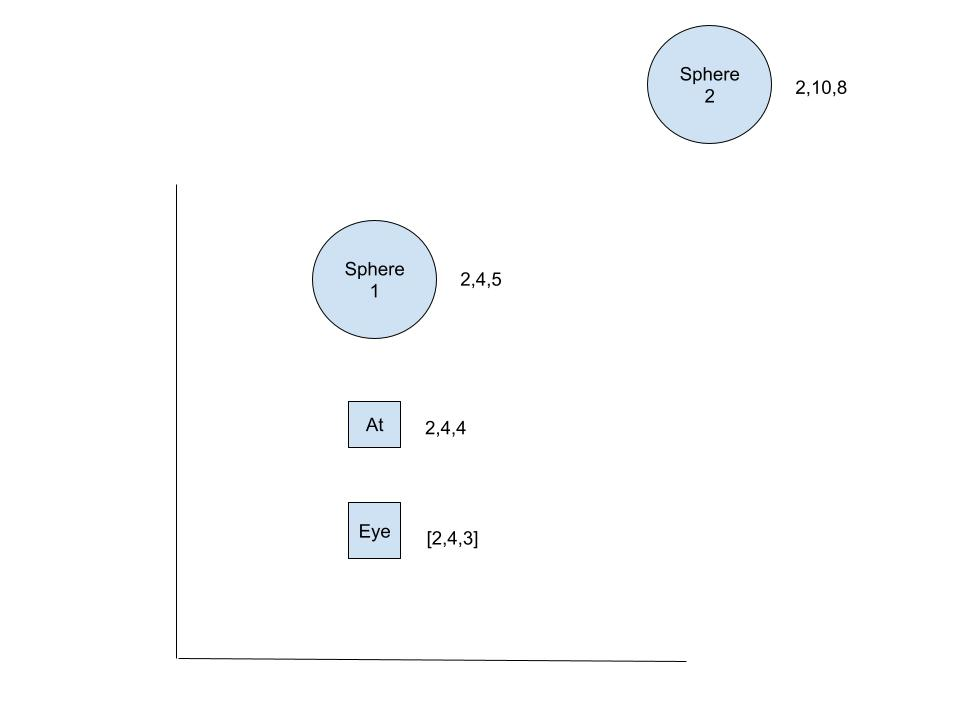
\includegraphics[scale=0.20, angle = 0]{img/yz_diag.jpg}
                        \end{center}
                    \end{figure}
                \item What is the distance to the near and far plane if they are set to bound the
                    objects as closely as possible? Describe the distance in numerical values and
                    explain it.

                    \begin{mdframed}
                        The near plane must be close enough
                        that no part of the closest object
                        crosses it, and the far plane must be
                        far enough that no part
                        of the farthest object crosses it.

                        For this scenario a near plane of 1 would
                        make sense since the near sphere is 2 units
                        from the eye, and has a radius of 1.

                        The far plane would need to be set
                        to 6, since it is 5 units away long
                        the look direction and 1 unit in radius.

                        We measure distance along the look direction
                        since this is what is used to define the near
                        and far planes rather than the euclidean distance
                        between the points.
                    \end{mdframed}
                    \break

                \item If we render this scene with a projection matrix, how many spheres will be seen
                    in each of the following cases? Why?
                    \begin{enumerate}
                        \item perspective(fovy=1°, aspect=1, zNear=1, zFar=100)
                            \begin{mdframed}
                                You would see only the first sphere. It is within
                                the near and far planes so that isn't an issue.

                                However the 1 degree field of view means that
                                only a sphere directly in line with or very close
                                to the look direction will be visible. The other
                                sphere is more than 30 degrees away from the look
                                direction meaining it won't be visible.
                            \end{mdframed}

                        \item perspective(fovy=175°, aspect=1, zNear=4, zFar=10)
                            \begin{mdframed}
                                In this case we would only see the far sphere.
                                The near sphere is closer than the nearplane,
                                and the fov is wide enough that the far sphere is
                                captured in it. In addition the
                                far plane is far enough away to capture the 
                                far sphere.
                            \end{mdframed}

                        \item perspective(fovy=60°, aspect=1, zNear=1, zFar=10)
                            \begin{mdframed}
                                I believe both spheres would be visible.
                                The near plane and far plane are far enough apart that
                                both spheres lie between them, and the fov is high
                                enough that the far sphere should be within the view
                                frustum.
                            \end{mdframed}
                    \end{enumerate}
            \end{enumerate}
    \end{enumerate}

    {\large Lighting}
    \begin{enumerate}
        \item Define the three components of light used in the Phong lighting model: diffuse,
            specular, and ambient.
            \begin{mdframed}
               The diffuse component is the light absorbed and scattered from an object
               in all directions. This happens when light hits a rough surface and bounces seemingly
               randomly.

               The specular component is the light which bounces in one particular direction.
               This happens when light hits a smooth surface and reflects.

               The ambient light is a representation of the light which bounces many times
               off the objects in the environment.

               In the lighting model the diffuse component is modeled via
               the cosine, the specular via the reflection, and the ambient
               is a constant added to the base light.
            \end{mdframed}

            \break
        \item Match the images below to the properties defined in the table. Write the image
            number in the correspondent table row.

            \begin{tabular}{|c|c|c|c|}
                \hline
                Diffuse Color & Specular Color & Specular Exponent & Image Number\\
                \hline
                Red & Black & Any & 7\\
                \hline
                Blue & Red & Small & 3\\
                \hline
                Blue & White & Big & 1\\
                \hline
                Dark Blue & Red & Medium-big & 10\\
                \hline
                Blue & Red & Big & 4\\
                \hline
                Blue & Black & Any & 2\\
                \hline
                Black & Red & Big Red & 9\\
                \hline
                Red & White & Small & 6\\
                \hline
                Red & White & Big & 8\\
                \hline
                Red & Blue & Big & 5\\
                \hline
            \end{tabular}

            \begin{mdframed}
                I am assuming that by big the table means that
                the p value is small, since the specular
                value is between 0 and 1, (clamped) raising it
                to a power will actually lower the value.
            \end{mdframed}

        \item Consider a scene with a single sphere of radius 1 centered at the origin (0,0,0).
            The sphere’s ambient coefficient is ka = RGB(0.1,0.1,0.1), diffuse coefficient kd =
            RGB(0.5,0.5,0.5), and specular coefficient ks = RGB(0.5,0.5,0.5), with specular ex-
            ponent s = 2. There is a light at position p1 = (0,2,0) with color c1 = RGB(1.0,
            0.0, 0.0). The camera is located at position p2 = (3,1,0). Calculate the Phong
            Illumination for the sphere fragment located at position p3 = (0,1,0).

            \begin{enumerate}
                \item Calculate the ambient portion of the color of this fragment.
                    \begin{mdframed}
                       The ambient coefficient is 0.1, meaning
                       the ambient light is $RGB(0.1, 0.1, 0.1) * RGB(1.0, 0.0, 0.0) = RGB(0.1, 0.0, 0.0)$.
                    \end{mdframed}

                \item Calculate the diffuse portion of the color of this fragment.
                    \begin{mdframed}
                        The diffuse component is calculated by taking
                        the dot product between the light direction and the normal,
                        then multiplying by the diffuse coefficient and the lighting
                        color.

                        \begin{displaymath}
                            n = [0, 1, 0]
                        \end{displaymath}
                        \begin{displaymath}
                            l = [0, 2, 0] - [0, 1, 0]
                            = [0, 1, 0]
                        \end{displaymath}
                        \begin{displaymath}
                            n \cdot l = 1
                        \end{displaymath}
                        \begin{displaymath}
                            c_l c_r = RGB(0.5, 0.0, 0.0)
                        \end{displaymath}
                    \end{mdframed}

                \item Calculate the specular portion of the color of this fragment.
                    \begin{mdframed}
                        
                        \begin{displaymath}
                            h = \frac{e + l}{||e + l||}
                        \end{displaymath}
                        \begin{displaymath}
                            h =\frac{[3, 0, 0] + [0, 1, 0]}{||e + l||}
                        \end{displaymath}
                        \begin{displaymath}
                            h = [3, 1, 0]/\sqrt{10}
                        \end{displaymath}
                        \begin{displaymath}
                            (h \cdot n)^p = (1/\sqrt{10})^2 = 1/10 = 0.1
                        \end{displaymath}
                        \begin{displaymath}
                            c = c_l * 0.1 = RGB(0.1, 0.0, 0.0)
                        \end{displaymath}
                    \end{mdframed}

                \item Calculate the total color of this fragment.
                    \begin{mdframed}
                        Since the terms were written as ambient and diffuse
                        coefficient, I will separate them out rather than add
                        the diffuse and ambient terms before multiplying by the
                        diffuse coefficient.

                        \begin{displaymath}
                            c = c_a + c_d + c_s = RGB(0.7, 0.0, 0.0)
                        \end{displaymath}
                    \end{mdframed}

                \item Now suppose the camera moves to p4 = (0,3,0). What is the total color of the
                    fragment?

                    \begin{mdframed}
                        Only the specular would change. 
                        \begin{displaymath}
                            h = \frac{e + l}{||e + l||}
                        \end{displaymath}
                        \begin{displaymath}
                            h =\frac{[0, 2, 0] + [0, 1, 0]}{||e + l||}
                        \end{displaymath}
                        \begin{displaymath}
                            h = [0, 3, 0]/3
                        \end{displaymath}
                        \begin{displaymath}
                            (h \cdot n)^p = (1)^2 = 1
                        \end{displaymath}
                        \begin{displaymath}
                            c = c_l * 0.1 = RGB(1.0, 0.0, 0.0)
                        \end{displaymath}

                        Meaning the new color is

                        \begin{displaymath}
                            c = c_a + c_d + c_s = RGB(1.6, 0.0, 0.0)
                            = RGB(1.0, 0.0, 0.0)
                        \end{displaymath}
                    \end{mdframed}
            \end{enumerate}

            \break
        \item Consider an orthographic scene with objects listed below being rendered at 5 x
            5 pixels with with the view plane at z=0 (near=0, far=99). Show the state of
            the z-buffer (with numbers) once these squares have been rendered (without using
            anti-aliasing or sub-sampling). Note that the pixels are drawn such that the z-buffer
            values are stored halfway between integers (look at the labels below the z-buffer).

            Red square with vertices: (0,0,1), (1,0,1), (1,1,1), (0,1,1)
            Green square with vertices: (2,2,2), (4,2,2), (4,4,2), (2,4,2)
            Blue square with vertices: (0,0,3), (4,0,3), (4,4,3), (0,4,3)

            \begin{figure}[ht]
                \begin{center}
                    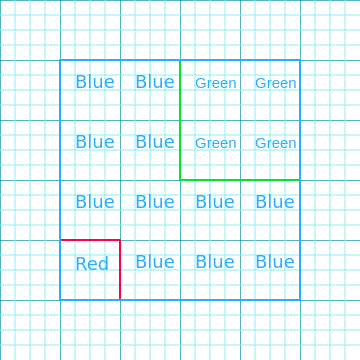
\includegraphics[scale=0.20, angle = 0]{img/zbuf.png}
                \end{center}
            \end{figure}
            \begin{mdframed}
                Here red refers to a value of 1, Blue a value of 3, and
                Green a value of 2. Everything else has a value
                of 99.
            \end{mdframed}

            \break
        \item Consider the following vertex and fragment shaders:
            {
                \hfuzz=50pt
                \begin{figure}[ht]
                    \begin{lstlisting}[language=C, gobble=24]
                        // Vertex Shader
                        uniform mat4 u_NormalMatrix;
                        uniform mat4 u_ModelMatrix;
                        uniform mat4 u_ViewMatrix;
                        uniform mat4 u_ProjectionMatrix;
                        attribute vec4 a_Position;
                        varying vec3 v_Position;
                        attribute vec4 a_Normal;
                        varying vec3 v_Normal;
                        void main() {
                            v_Normal = normalize(vec3(u_NormalMatrix * a_Normal));
                            v_Position = vec3(u_ModelMatrix * a_Position);
                            gl_Position = u_ProjectionMatrix *
                            u_ViewMatrix *
                            u_ModelMatrix *
                            a_Position;
                        }; 
                    \end{lstlisting}
                    \begin{lstlisting}[language=C, gobble=24]
                        // Fragment Shader
                        varying vec3 v_Position;
                        varying vec3 v_Normal;
                        uniform vec3 u_LightPos;
                        uniform vec3 u_LightColor;
                        void main() {
                            vec3 l = normalize(u_LightPos - v_Position);
                            float nDotL = max(dot(l, v_Normal), 0.0);
                            gl_FragColor = vec4(u_LightColor * nDotL);
                        }
                    \end{lstlisting}
                \end{figure}
            }

            \begin{enumerate}
                \item In the vertex shader, what is the normal matrix and why do we need to multiply
                    it by the normal vector?
                    \begin{mdframed}
                        The normal matrix is the model matrix
                        but without translation. We use
                        it to ensure the normals are transformed
                        to match the models orientation.
                    \end{mdframed}

                \item In the vertex shader, why do we multiply the vertex position by the model
                    matrix?

                    \begin{mdframed}
                        The model matrix will convert the local coordinates
                        of the object relative to its center to the world
                        coordinates. Basically the model matrix stores where
                        the object is and how it is oriented relative to all the
                        other objects in the world, and we use it to convert
                        our vertex positions to be relative to all the other
                        objects.
                    \end{mdframed}

                \item What is the fragment shader computing?
                    \begin{mdframed}
                        The fragment shader computes the light direction,
                        then takes the dot product with the surface normal. This
                        is a lambertian diffuse lighting component meaning
                        it is computing diffuse lighting.
                    \end{mdframed}
            \end{enumerate}
    \end{enumerate}

    {\large Readings}
    \begin{enumerate}
        \item What are the three items of information required to specify the viewing direction? Describe
            each one of them.
            \begin{mdframed}
                The first is the eye position. This is the position of the camera
                and the origin of our view.

                The second is the target to look at. Usually this is a world space point
                that the camera will look at, but this could also just be a look direction
                which gets added to the camera position. This specifies what line will
                lie in the center of the camera's view.

                The first two together actually leave a degree of freedom
                to rotate, so the last component specifies the up direction.
                Essentially if we rotate the view about the line specifying
                the look direction the first two parameters are satisfied, but
                by taking a direction orthogonal (ish), to the look direction
                we can map that to some static point and specify a single
                linear transformation.

                Essentially the orthogonal component of the up direction will
                get mapped to the top of the screen.
            \end{mdframed}

        \item Define a view matrix and describe the method that can be used (according to the book) to
            calculate it in Javascript?

            \begin{mdframed}
                A view matrix is a series of translations and rotations
                which places the eye at the origin, the point 1 unit in the
                look direction at the point $0,0,1$ and the up direction
                at $0,1,0$.

                In javascript we can use the provided lookAt function,
                which takes an eye position, an up vector, and an at
                point which is specified in world space, ie:
                at $=$ eye $ + $ look direction.

                \begin{lstlisting}[language=C, gobble=16]
                   var mat = new Matrix4(); 
                   mat.setLookAt(ex, ey, ez,
                                 at_x, at_y, at_z,
                                 up_x, up_y, up_z);
                \end{lstlisting}
            \end{mdframed}

            \break
        \item What is the difference between orthographic projection and perspective projection? What methods
            can be used to calculate the orthographic projection? And the perspective projection? Explain
            the arguments of both the methods.

            \begin{mdframed}
                Orthographic projections do not divide by the
                depth, meaning planes parallel to the
                camera view direction stay parallel in
                the final image.

                Perspective projections divide by the depth,
                meaining objects further away from the camera
                look smaller and straight lines can
                become curved.

                Orthographic projections are generally specified
                by giving a bounding box in terms of left,
                right, near, and far planes. You could
                do something like aspect ratio plus near
                and far but this is fairly uncommon since
                orthographic projections are usually used with
                a top left origin.

                Perspective projections are usually specified
                using fov, aspect ratio, near, and far.
                The fov, alongside the near and far planes
                are used to specify how dramatic the perspective
                correction will be. It is possible to specify
                a perspective frustum using left, right,
                near and far, but this is uncommon since
                changing the near and far planes will change
                the resulting image in an unintuitive way.

                Generally speaking perspective will produce
                more immersive and realistic images, while orthographic
                projections are used when precision and exact sizing is
                needed. So orthographic is the default in many CAD programs,
                while perspective is the default in game engines.
            \end{mdframed}

        \item Describe the three major types of light sources: directional, point and ambient.

            \begin{mdframed}
                Light is defined by the direction from the surface
                to the light source.

                Directional lights use a constant direction, these
                lights act like points infinitely far away.

                Point lights are points in space. meaning the direction
                changes as you move the surface.

                Ambient light is the light which we imagine has bounced off
                of many objects and suffuses the scene. This is usually
                done by just adding a constant light value to the final light.
                This type of light has no direction and is constant for all
                surfaces.
            \end{mdframed}

            \break
        \item Explain ambient reflection. Provide the equation that models this reflection and draw a figure
            illustrating it.

            \begin{mdframed}
                Ambient reflection can be modeled as a constant. 

                \begin{displaymath}
                    c = c_a
                \end{displaymath}

                The diagram shows light hitting the shape from
                all directions equally.
            \end{mdframed}
            \begin{figure}[ht]
                \begin{center}
                    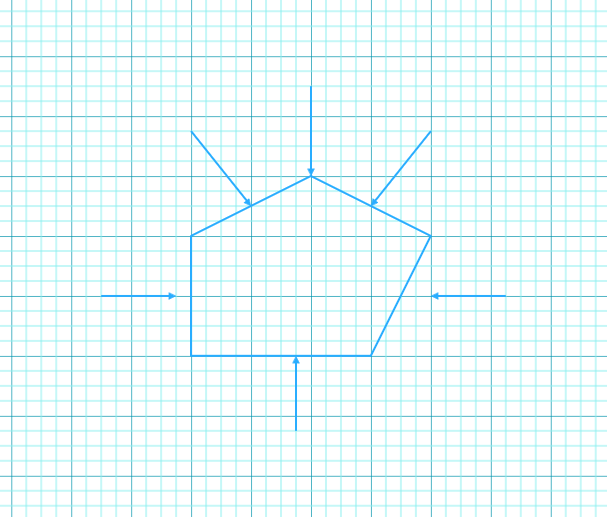
\includegraphics[scale=0.20, angle = 0]{img/amb.png}
                \end{center}
            \end{figure}

        \item Explain diffuse reflection. Provide the equation that models this reflection and draw a figure
            illustrating it.
            \begin{mdframed}
                Diffuse reflection is the light which hits the surface
                and scatters equally in all directions. It is proportional
                only the the amount the surface faces the light.

                \begin{displaymath}
                    c = c_r(n \cdot l)
                \end{displaymath}

                Where $c_r$ is the diffuse color, $n$ is the
                surface normal, and $l$ is the light direction.

                The image shows light hitting a surface and scattering
                in all directions.
            \end{mdframed}
            \begin{center}
                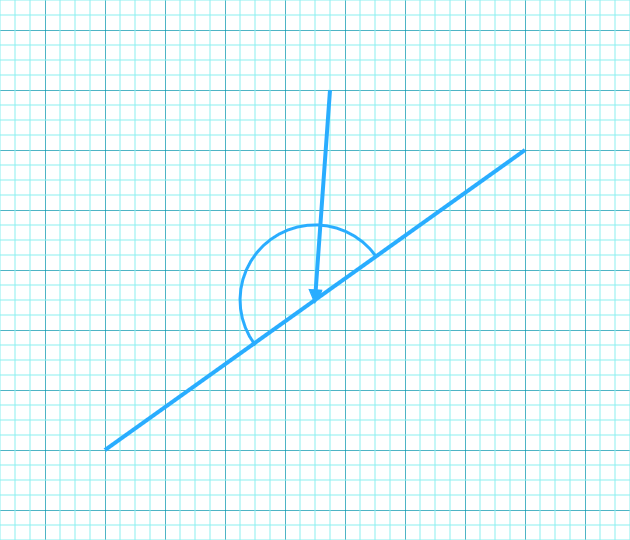
\includegraphics[scale=0.20, angle = 0]{img/diffuse.png}
            \end{center}

        \item What is a surface normal? How many normals are there in a surface? Draw a cube and the
            normals of all of its vertices.

            \begin{mdframed}
                The derivative of a surface at a point
                gives a plane. This plane is effectively the
                normal of the surface.

                This is not obvious at first since we also see the
                normal vector as a vector which points directly away
                from the surface, however for every 3D vector
                there is exactly 1 3D plane.

                \begin{displaymath}
                   \begin{bmatrix}
                        a\\ 
                        b\\
                        c
                   \end{bmatrix} 
                   \cdot
                   \begin{bmatrix}
                        x\\ 
                        y\\
                        z
                   \end{bmatrix}
                   + 1 = 0
                \end{displaymath}

                Is equivalent to

                \begin{displaymath}
                    ax + by + cz + 1 = 0
                \end{displaymath}

                Which is a general plane equation.

                For any given surface we can take
                the normal at any point, however for surfaces
                which are composed of triangles there is
                1 surface normal per triangle.

                That means for a cube there are 6 distinct
                normals corresponding to the 6 distinct
                planes which make up the polyhedron.

                At a vertex we have two options. We could
                say the normals point directly away from the
                center of the cube, which implies the
                triangles are an approximation of some
                smooth shape, or we can say that there
                are multiple normals which are associated with
                each face which implies the polyhedron is the
                actual shape and not an approximation.

                For the sake of this exercise here are the normals
                where I take the cube to be an approximation of a
                sphere.
            \end{mdframed}
            \begin{center}
                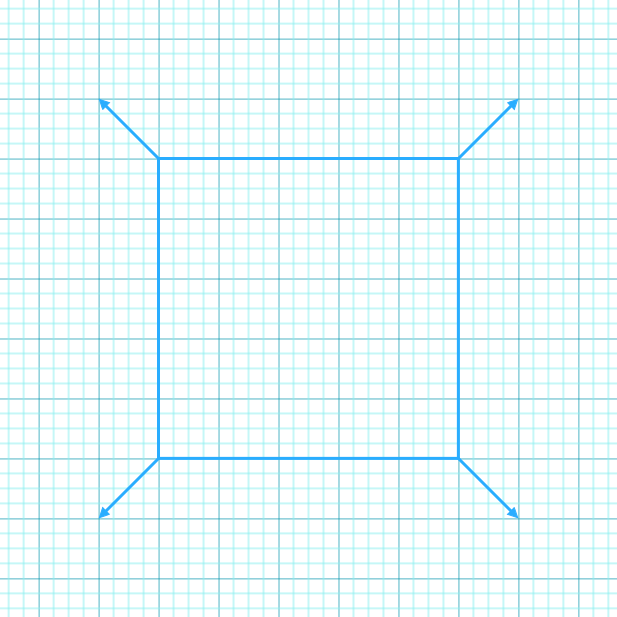
\includegraphics[scale=0.16, angle = 0]{img/norm.png}
            \end{center}
    \end{enumerate}

\end{document}
